\documentclass[12pt]{article}
\usepackage[utf8]{inputenc}
\usepackage{graphicx}
\usepackage{amsmath}
\usepackage{cite}
\title{
	{
\includegraphics[scale=0.3]{university.png}}\\
	{\large Amirkabir University of Technology}\\
	{Simulation report on our selected paper entitled "A Scalable Approach for Service Chain Mapping With Multiple SC Instances in a Wide-Area Network"}\\
	}
\author{Milad Khademi, Ali Zamani}
\date{30 June 2018}

\begin{document}


\maketitle

\newpage

\tableofcontents

\newpage

\section{Introduction}
 
Network Function Virtualization (NFV) aims to simplify service deployment using Virtual Network Functions (VNFs). Service deployment involves placement of VNFs and in-sequence routing of traffic flows through VNFs comprising a Service Chain (SC). The joint VNF placement and traffic routing is called SC mapping. In a Wide-Area Network (WAN), where several traffic flows, generated by many distributed node pairs, require the same SC; a single instance (or occurrence) of that SC might not be enough. SC mapping with multiple SC instances for same SC is a very complex problem, since sequential traversal of VNFs has to be maintained while accounting for traffic flows in various directions \cite{second}.

\subsection{Network Function Virtualization}
Traditionally, communication networks have deployed network services through proprietary hardware appliances (e.g., network functions such as firewalls, NAT, etc.) which are statically configured. With rapid evolution of applications, networks require agile and scalable service deployment.

Network Function Virtualization (NFV) \cite{first} offers a solution for an agile service deployment. NFV envisions traditional hardware functionality as software modules called Virtual Network Functions (VNFs). VNFs can be run on commercial-off-the-shelf hardware such as servers and switches in datacenters (DCs), making service deployment agile and scalable.
\subsection{Service Chain}
When several network functions are configured to provide a service, we have a “Service Chain”. The term “service chain” is used “to describe the deployment of such functions, and the network operator’s process of specifying an ordered list of service functions that should be applied to a deterministic set of traffic flows”. So, a “Service Chain” (SC) specifies a set of network functions configured in a specific order. With NFV, we can form SCs where VNFs are configured in a specific sequence that minimizes the bandwidth usage in the network \cite{third}. 

In Table \ref{table:1} we show some well-known Service Chains (SCs). \\
\begin{table}[t!]
\centering
\begin{tabular}{|c c|} 
 \hline
 Service Chains & Chained VNFs \\ [0.5ex] 
 \hline 
 Web Service & NAT-FW-TM-WOC-IDPS\\ 
VoIP &NAT-FW-TM-FW-NAT \\
 Video Streaming & NAT-FW-TM-VOC-IDPS \\
 Online Gaming&NAT-FW-VOC-WOC-IDPS\\[1ex] 
 \hline
\end{tabular}
\caption{Service Chain Requirements; Network Address Translator (NAT), Firewall (FW), Traffic Shaper (TM), WAN Optimization Controller (WOC), Intrusion Detection and Prevention System (IDPS), Video Optimization Controller (VOC).}
\label{table:1}
\end{table}

\subsection{Service Chain Mapping Issues}
Unfortunately, since VNFs in a single SC may need to be traversed by several distinct traffic flows (i.e., flows requested by multiple geographically-distributed node pairs) in a specific sequence, it becomes difficult to improve network resource utilization.

For example, consider Figure 1(a) and 1(b), where three traffic requests $r_1$ (from node 4 to 13), $r_2$ (from node 6 to 3), and $r_3$ (from node 14 to 1) demand SC $c_1$ composed of VNF1, VNF2, and VNF3 (to be traversed in this order VNF1$\rightarrow$ VNF2  $\rightarrow$ VNF3).

In Figure 1(a), if we consider only one mapping occurrence (or instance) for SC $c_1$, then some traffic flows (in our example, $r_3$ and $r_2$) will be ineffectively routed over long paths. Instead, as shown in Figure 1(b), if we use two SC instances for the same SC, we can improve network resource utilization, at the expense of a larger number of VNFs to be deployed (or replicated) in the network to serve the same SC. This results in a more complex problem when, in a Wide-Area Network (WAN), a large number of distributed node pairs generate traffic flows, creating heavy traffic demands. Our objective in this work is to reduce the network resource consumption for a WAN with heavy traffic demands.
\begin{figure}[t!] \label{fig:1}
  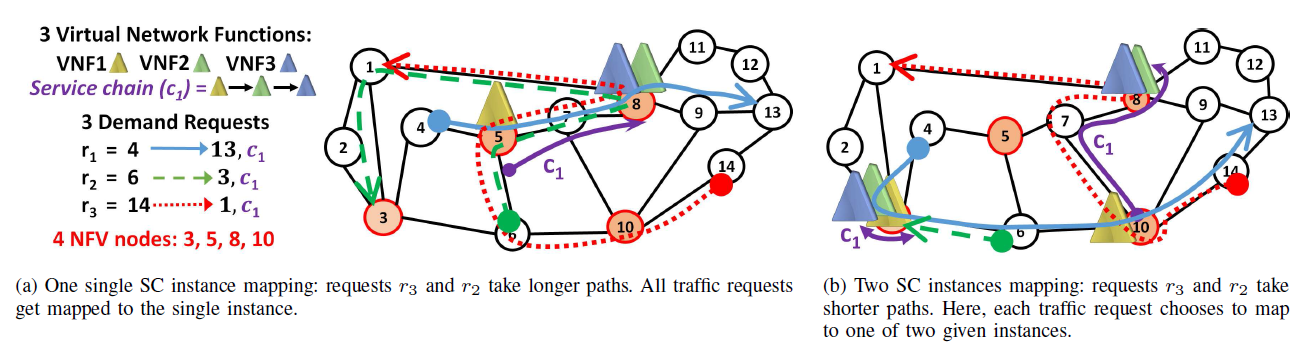
\includegraphics[width=\linewidth]{fig1.png}
  \caption{Deploying more SC occurrence mappings reduces network resource consumption.}
\end{figure}

So the question is: how many SC instances for the same SC are required for optimal network resource utilization?

A possible (trivial) solution to the problem of SC mapping in case of multiple node pairs requiring the same SC is to use one single instance that would most likely lead to host SCs at a single node (e.g., a DC) which is centrally located in the network. However, traffic flows may have to take long paths to reach the node hosting the SC, which will result in a high network resource consumption.

The other extreme case would be to use a distinct SC mapping per node pair (in other words, the number of SC instances is equal to the number of traffic node pairs). Now, we can achieve optimal network resource utilization as each node pair will use an SC effectively mapped along a shortest path in the network. However, this approach will increase the network orchestration overhead and increase capital expenditure, as there will be a large number of replicated VNF instances across nodes. To reduce excessive VNF replication, we bound the maximum number of nodes hosting VNFs.

Intuitively, the number of SC instances for a good solution will be a value between these two extremes. This solution will minimize the network resource utilization while not excessively increasing the number of nodes hosting VNFs \cite{Fourth}.
\section{System Model and Problem Formulation}
An operator’s network provides multiple services, and each service is realized by traversing a Service Chain (SC). To provide multiple services, the operator has to map corresponding SCs into network.
\subsection{System Model}
\begin{table}[t!]
\centering
\begin{tabular}{|c l|} 
 \hline
 Notations & Descriptions \\ [0.5ex] 
 \hline 
 $G$ & Physical topology of backbone network $G = (V,L)$\\ 
& with $V$: node set and $L$: link set\\ 
 $V^{NFV}$ & $ \subseteq V$ Set of nodes that can host VNFs (NFV nodes) \\
 $I_c$ & Number of instances for SC $c$ \\
 $K$& Maximum number of NFV nodes to host VNFs\\
 $F$&Set of VNFs, indexed by $f$\\
 $R_f$& Maximum number of replicas of VNF $f$\\
 $n^{core}$&Number of CPU cores present in a NFV node\\
 $n^{core}_f$& Number of CPU cores per Gbps for function $f$\\
 $C$& Set of chains, indexed by $c$\\
 $n_c$& Number of VNFs in SC $c$\\
 $SD$&Set of source-destination $(v_s, v_d)$ pairs\\
 $SD_c$&Set of source-destination $(v_s, v_d)$ pairs for SC $c$\\
 $D_{sd}^c$&Traffic demand between $v_s$ and $v_d$ for SC $c$\\
 $\sigma_i (c)$& ID of $i$th VNF in SC $c$, where $f_{\sigma_i (c)} \in F$\\
 $T_{fi}^c$& VNF ID ($f$) of the $i$th VNF in SC $c$\\[1ex] 
 \hline
\end{tabular}
\caption{Notations Descriptions}
\label{table:2}
\end{table}
Given a network topology, capacity of links, a set of network nodes with NFV support (NFV nodes), compute resources at NFV nodes, maximum number of NFV nodes that can be used, traffic flows for source-destination pairs requiring a specific SC with a certain bandwidth demand, a set of VNFs, and a set of SCs, we determine the placement of VNFs and corresponding traffic routing to minimize network resource (bandwidth) consumption. Note that VNFs can be shared among different SCs.

Table \ref{table:3} describes the input parameters used. To facilitate model formulation and discussion, we propose the concept of configuration ($\hat{\gamma}$). We use the following notation for SC representation. Each SC, denoted by $c$, is characterized by an ordered set of $n_c$ functions:
\begin{equation}
[\textrm{SC}\ c]\quad f_{\sigma_1 (c)}\prec f_{\sigma_2 (c)}\prec \cdots \prec f_{\sigma_{n_c} (c)}
\end{equation}
Each deployment of SC $c$ is defined by a set of VNF locations, a set of paths, from location of first VNF to location of last VNF, and set of traffic flows traversing this deployment.

We generate a set of \emph{SC configurations} where each configuration ($\hat{\gamma}$) is associated with a potential provisioning of a SC $c$, i.e., with a potential node placement of its functions and a potential subset of traffic flows from $SD_c$. Let $\hat{\Gamma}$ be the set of configurations, and $\hat{\Gamma}_c$ be the subset of configurations associated with service chain $c\in C$:\ \   $\hat{\Gamma}=\bigcup_{c\in C} \hat{\Gamma}_c$

Potential set of configurations for a SC $c$ is given by:
\begin{equation}
\hat{\Gamma}_c=\sum_{sd=1}^{N_{SD_c}} \left(
    \begin{array}{c}
      N_{SD_c} \\
      sd
    \end{array}
  \right)
\times \{ N_{V^{NFV}} \}^{n_c}
\times  (P_{paths})^{n_c -1}
\end{equation}
where $sd$ is the number of source-destination $(v_s, v_d)$ pairs using a configuration, $N_{SD_c}$ gives the number of source-destination $(v_s, v_d)$ pairs for SC $c$, $N_{V ^{NFV}}$ gives the number of NFV nodes and $P_{paths}$ refers to the number of paths from the location of $f_{\sigma_i (c)}$ to the location of $f_{\sigma_{i+1} (c)}$.

A chain configuration ($\hat{\gamma}$) is characterized by the following parameters:
\begin{table}[t!]
\centering
\begin{tabular}{|c l|} 
 \hline
 Notations & Descriptions \\ [0.5ex] 
 \hline
 $z_{\hat{\gamma}}$ & 1 if configuration $\hat{\gamma}$ is selected; 0 otherwise\\ 
 $x_{vf}$ & 1 if function $f$ is located in $v$; 0 otherwise \\
 $y_{\ell}^{f_1 (c),sd}$ & 1 if $\ell$ is on path from $v_s$ to location of first VNF in $c$; 0 otherwise \\
 $y_{\ell}^{f_{n_c} (c),sd}$& 1 if $\ell$ is on path from $v_d$ to location of first VNF in $c$; 0 otherwise\\
 $h_v$&1 if $v$ is used as a location for a VNF; 0 otherwise\\[1ex] 
 \hline
\end{tabular}
\caption{Variables}
\label{table:3}
\end{table}

\begin{itemize}
  \item Traffic flows: $\delta^{\hat{\gamma}}_{sd}= 1$ if $(v_s, v_d)$ uses configuration $ \hat{\gamma}$; 0 otherwise.
  \item Location of functions: $a^{\hat{\gamma}}_{vi} = 1$ if $i$th function $f_i \in c$ is located in $v$ in configuration $\hat{\gamma}$; 0 otherwise.
  \item Connectivity of locations: path from location of current VNF to next VNF in SC $c$. If link $\ell$ is used in the path from location of $f_{\sigma_i (c)}$ to location of $f_{\sigma_{i+1}(c)}$, then $b_{il}^{\hat{\gamma}} = 1$; 0 otherwise.\\
 
\end{itemize}
\subsection{Problem Formulation to an ILP}
We precompute $\hat{\Gamma}$, which is an input for our ILP model. ILP selects the best configuration ($\hat{\gamma}$) based on other input parameters and constraints, and computes the route from $v_s$ (source) to first VNF of $c$ and from last VNF of $c$ to $v_d$ (destination) for each source-destination $(v_s, v_d)$ pair.

\textbf{Variables:} See Table 2.

\textbf{Objective:} Minimize bandwidth consumed:
\begin{equation}
\begin{split}
\sum_{c \in C}\sum_{\hat{\gamma}\in \hat{\Gamma}_c}
\overbrace{(\sum_{(s, d)\in SD} D^{c}_{sd})}^{\textrm{Overall traffic  using $c$}} \quad
\overbrace{(\sum_{\ell \in L} \sum_{i \in I} \delta_{sd}^{\hat{\gamma}} b_{i\ell}^{\hat{\gamma}})}^{\textrm{Number of links on the route of $c$}}
z_{{\hat{\gamma}}} \\ +\sum_{c \in C} 
\sum_{\ell \in L}\sum_{(s, d)\in SD}D_{sd}^{c}(y_{\ell}^{f_{1} (c),sd}+y_{\ell}^{f_{n_c} (c),sd})
\end{split}
\end{equation}
Total bandwidth consumed in placing multiple SCs depends on configurations ($\hat{\gamma}$’s) selected for each SC $c$. Each $\hat{\gamma}$ for $c$ locates VNFs of $c$ and gives the route to traverse these VNF locations. So, bandwidth consumed when going from $v_s$ to $v_d$ and traversing the SC depends on selected $\hat{\gamma}$. Bandwidth consumed depends on the number of links, i.e., number of hops in path from $v_s$ to $v_d$.\\
\textbf{Constraints:}

\begin{equation} 
\sum_{\hat{\gamma}\in \hat{\Gamma}_c}z_{{\hat{\gamma}}}\leq I_c \quad \quad c\in C
\end{equation}
\begin{equation}
\sum_{c \in C}\sum_{\hat{\gamma}\in \hat{\Gamma}_c}\sum_{i=1}^{n_c}T_{fi}^{c}a_{vi}^{\hat{\gamma}}z_{{\hat{\gamma}}}\leq Mx_{vf} \quad \quad f\in F, v\in V^{NFV}
\end{equation}
\begin{equation}
\sum_{c \in C}\sum_{\hat{\gamma}\in \hat{\Gamma}_c}\sum_{i=1}^{n_c}T_{fi}^{c}a_{vi}^{\hat{\gamma}}z_{{\hat{\gamma}}}\geq x_{vf}\quad \quad f\in F, v\in V^{NFV}
\end{equation}
\begin{equation}
\sum_{v \in V^{NFV}} x_{vf}\leq R_{f} \quad \quad f\in F
\end{equation}
\begin{equation}
Mh_v \geq \sum_{f \in F} x_{vf}\geq h_{v} \quad \quad  v\in V^{NFV}
\end{equation}
\begin{equation}
\sum_{v \in V^{NFV}} h_v \leq K
\end{equation}
\begin{equation}
\sum_{c \in C}\sum_{\hat{\gamma}\in \hat{\Gamma}_c}\sum_{(v_s, v_d)\in SD} D^{c}_{sd}\delta_{sd}^{\hat{\gamma}}\times (\sum_{f \in F}\sum_{i=1}^{n_c}T_{fi}^{c}n_{f}^{CORE}a_{vi}^{\hat{\gamma}})z_{\hat{\gamma}}\leq N^{CORE} \quad v\in V_{NFV}
\end{equation}
\begin{equation}
\sum_{c \in C}\sum_{(v_s, v_d)\in SD} D^{c}_{sd}\times (y_{\ell}^{f_{1} (c),sd}+y_{\ell}^{f_{n_c} (c),sd}+\sum_{\hat{\gamma}\in \hat{\Gamma}_c}\delta_{sd}^{\hat{\gamma}}z_{\hat{\gamma}}\sum_{i=1}^{n_c -1}b_{i\ell}^{\hat{\gamma}}) \leq CAP_{\ell} \quad \ell \in L
\end{equation}
\begin{equation}
\sum_{\hat{\gamma}\in \hat{\Gamma}_c}\delta_{sd}^{\hat{\gamma}}z_{\hat{\gamma}}=1\quad \quad c\in C, (v_s,v_d)\in SD : D_{sd}^{c}>0
\end{equation}
Constraints (4) guarantee that we select exactly $I_c$ configurations for SC $c$ and force $c$ to have $I_c$ instances. Each $\hat{\gamma}$ is associated with a set of $a_{vi}^{\hat{\gamma}}$ required to be consistent with $x_vf$ , which is resolved by Eqs. (4), (5) where $T_{c}^{fi}$ is to find the VNF f at sequence i in SC $c$. Eq. (6) is used to limit the number of VNF replicas. Eq. (7) is used to keep track of NFV nodes used for hosting VNFs while Eq. (8) limits the number of NFV nodes allowed to host VNFs. Constraints (9) ensure that each NFV node has a sufficient number of CPU cores for hosting $f$. Eq. (10) constrains link capacity. Eq. (11) enforces that, for each source-destination pair $(v_s, v_d)$ requesting SC $c$, there is exactly one configuration $\hat{\gamma}$.

\textbf{Route from} \textbf{$v_s$} \textbf{to first function location:}
\begin{equation}
\sum_{\hat{\gamma}\in \hat{\Gamma}_c}\delta_{sd}^{\hat{\gamma}}a_{v_s ,1}^{\hat{\gamma}}z_{\hat{\gamma}}+\sum_{\ell \in \omega^{+} (v_s)}y_{\ell}^{f_1 (c),sd}=1 \quad \quad c \in C, (v_s, v_d) \in SD: D_{sd}^{c}>0
\end{equation}
\begin{equation}
\begin{split}
\sum_{\hat{\gamma}\in \hat{\Gamma}_c}\delta_{sd}^{\hat{\gamma}}a_{1}^{\hat{\gamma}}z_{\hat{\gamma}}-\sum_{\ell \in \omega^{-} (v)}y_{\ell}^{f_1 (c),sd} \leq 0 \\
 \quad \quad c \in C, (v_s, v_d) \in SD: D_{sd}^{c}>0 \ \ v\in V^{NFV} \backslash  \{v_s\}
\end{split}
\end{equation}
\begin{equation}
\begin{split}
\sum_{\hat{\gamma}\in \hat{\Gamma}_c}\delta_{sd}^{\hat{\gamma}}a_{1}^{\hat{\gamma}}z_{\hat{\gamma}}+\sum_{\ell \in \omega^{+} (v)}y_{\ell}^{f_1 (c),sd}-\sum_{\ell \in \omega^{-} (v)}y_{\ell}^{f_1 (c),sd}=0 \\
  c \in C, (v_s, v_d) \in SD: D_{sd}^{c}>0, \ \ v\in V^{NFV} \backslash  \{v_s\}
\end{split}
\end{equation}
\begin{equation}
\begin{split}
\sum_{\ell \in \omega^{+} (v)}y_{\ell}^{f_1 (c),sd}-\sum_{\ell \in \omega^{-} (v)}y_{\ell}^{f_1 (c),sd}=0 \\
  c \in C, (v_s, v_d) \in SD: D_{sd}^{c}>0, \ \ v\in V \backslash (V^{NFV} \cup   \{v_s\})
\end{split}
\end{equation}
We assume that a unique route exists from $v_s$ to first VNF location. This is imposed by selecting exactly one outgoing link from $v_s$ unless first VNF is located at $v_s$. We account for these scenarios using Eq. (13). To find the route from $v_s$ to first VNF, flow conservation needs to be enforced at the intermediate nodes which may or may not have NFV support. Eqs. (14) and (15) enforce flow-conservation constraints at nodes with and without NFV support, respectively.

\textbf{Route from last function location to $v_d$:}
\begin{equation}
\sum_{\hat{\gamma}\in \hat{\Gamma}_c}\delta_{sd}^{\hat{\gamma}}a_{v_d , n_c}^{\hat{\gamma}}z_{\hat{\gamma}}+\sum_{\ell \in \omega^{-} (v_d)}y_{\ell}^{f_{n_c} (c),sd}=1 c \in C, (v_s, v_d) \in SD: D_{sd}^{c}>0
\end{equation}
\begin{equation}
\begin{split}
\sum_{\hat{\gamma}\in \hat{\Gamma}_c}\delta_{sd}^{\hat{\gamma}}a_{v_d , n_c}^{\hat{\gamma}}z_{\hat{\gamma}}-\sum_{\ell \in \omega^{+} (v)}y_{\ell}^{f_{n_c} (c),sd}\leq 0 \\
 c \in C, (v_s, v_d) \in SD: D_{sd}^{c}>0, v \in V^{NFV} \backslash \{v_d\}
\end{split}
\end{equation}

\begin{equation}
\begin{split}
\sum_{\hat{\gamma}\in \hat{\Gamma}_c}\delta_{sd}^{\hat{\gamma}}a_{v_d , n_c}^{\hat{\gamma}}z_{\hat{\gamma}}-\sum_{\ell \in \omega^{+} (v)}y_{\ell}^{f_{n_c} (c),sd}+\sum_{\ell \in \omega^{-} (v)}y_{\ell}^{f_{n_c} (c),sd}=0 \\
 c \in C, (v_s, v_d) \in SD: D_{sd}^{c}>0, v \in V^{NFV} \backslash \{v_d\}
\end{split}
\end{equation}

\begin{equation}
\begin{split}
\sum_{\ell \in \omega^{+} (v)}y_{\ell}^{f_{n_c} (c),sd}+\sum_{\ell \in \omega^{-} (v)}y_{\ell}^{f_{n_c} (c),sd}=0 \\
 c \in C, (v_s, v_d) \in SD: D_{sd}^{c}>0, v \in V^{NFV} \backslash \{v_d\}
\end{split}
\end{equation}
Eq. (17) selects one incoming link to $v_d$ to ensure a route to $v_d$. For cases where last VNF is placed at destination node, we use Eq. (18). Eqs. (19) and (20) enforce flow conservation at nodes with and without NFV support, respectively.
\section{Simulation}
\subsection{Simulation Parameters Declaration}
We tested our optimization process on a 14-node NSFNET WAN topology as shown in Figure 2. To simplify the simulation, we considered a traffic matrix which consists of 5 demands with just one type of Service Chain (Refer to Table \ref{table:4}). Just 4  nodes can be made NFV nodes. The link capacities are 1Tbps. Each traffic flow demand is 1 Gbps. Compute resource (CPU) at each NFV node is 100 cores per node. All other simulation parameters are shown in Table \ref{table:5}.
\begin{figure}[t!]
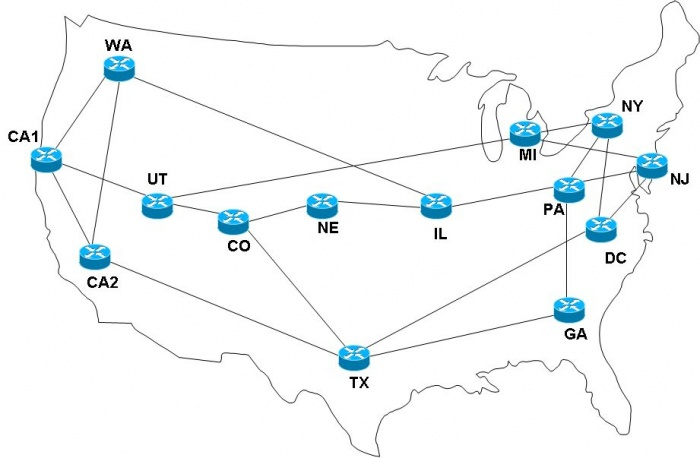
\includegraphics[scale=0.5]{nsfnet.jpg}
\caption{14-node NSFNET WAN topology.}
\end{figure}
\begin{table}[t!]
\centering
\begin{tabular}{|c c c c c|} 
 \hline
 Number&Source & Destination & Demanded SC&  Bandwidth \\ [0.5ex] 
 \hline
$1$&Washington & NewJersey & Web Service& $1Gbps$\\ 
$2$&Texas & Michigan & Web Service& $1Gbps$\\
$3$&WashingtonDC & Washington & Web Service& $1Gbps$\\
$4$&California2 & Michigan & Web Service& $1Gbps$\\
$5$&California1 & NewYork & Web Service& $1Gbps$\\[1ex] 
 \hline
\end{tabular}
\caption{Traffic demands ($D_{sd}^{c})$}
\label{table:4}
\end{table}

\begin{table}[t!]
\centering
\begin{tabular}{|c c|} 
 \hline
 Parameter & Value \\ [0.5ex] 
 \hline 
 $G$ &It is shown in Figure 2\\ 
 $V^{NFV}$ & All nodes can be NFV node  \\
 $I_c$ &  $4$ \\
 $K$&$4$ \\
 $F$& \{NAT, FW, TM, WOC, IDPS\} \\
 $R_f$& $2$\\
 $n^{core}$ & $100$\\
 $n^{core}_f$ & $[1 \ 1 \ 1 \ 1\ 1]$\\
 $C$& \{Web Service \} \\
 $n_c$& $5$\\
 $SD$&It is shown in Table \ref{table:4}\\
 $SD_c$&It is shown in Table \ref{table:4}\\
 $D_{sd}^c$&It is shown in Table \ref{table:4}\\
 $\sigma_i (c)$& ID of $i$th VNF in SC $c$, where $f_{\sigma_i (c)} \in F$\\
 $T_{fi}^c$& VNF ID ($f$) of the $i$th VNF in SC $c$\\[1ex] 
 \hline
\end{tabular}
\caption{Simulation Parameters}
\label{table:5}
\end{table}
\subsubsection{Precompution Step}
As we have stated in previous Section we should precompute $\hat{\Gamma}$, which is an input for our ILP model. Then ILP selects the best configuration ($\hat{\gamma}$) based on other input parameters and constraints. We map all network nodes which are the name of States in USA (Refer to Figure 2) to a number which is shown in Table \ref{table:6}. Table \ref{table:7} shows 10 different configurations ($\hat{\gamma}$) which we have computed manually.
\begin{table}[t!]
\centering
\begin{tabular}{|c c|} 
 \hline
 State & Number \\ [0.5ex] 
 \hline 
 Washington&$1$\\ 
 California1&$2$ \\
 California2&$3$ \\
 Utah&$4$ \\
 Colorado&$5$ \\
 Utah&$6$ \\
 Texas&$7$ \\
 Nebraska&$8$ \\
 Illinois&$9$ \\
 Pennsylvania&$10$ \\
 Georgia&$11$ \\
 NewYork&$12$ \\
 NewJersey& $13$\\
 WashingtonDC&$14$\\[1ex] 
 \hline
\end{tabular}
\caption{Each USA State and its corresponding number}
\label{table:6}
\end{table}

\begin{table}[t!]
\centering
\begin{tabular}{|c c|} 
 \hline
 Number & Configuration  \\ [0.5ex] 
 \hline
 $1$st& $3 (f_1,f_2) \rightarrow 6 \rightarrow 5(f_3) \rightarrow 7 \rightarrow 8(f_4)  \rightarrow 9 \rightarrow 10(f_5)$\\ [2ex]

 $2$nd&$ 3(f_1) \rightarrow 6 \rightarrow 10(f_2,f_3) \rightarrow 9 \rightarrow 8(f_4) \rightarrow 7 \rightarrow 5(f_5)$\\ [2ex]

 $3$rd& $3(f_1) \rightarrow 2 \rightarrow 4 \rightarrow 5(f_2,f_3) \rightarrow 7 \rightarrow8(f_4) \rightarrow 9 \rightarrow 10(f_5)$ \\ [2ex]

 $4$th&$8(f_1)\rightarrow 7 \rightarrow 5(f_2)\rightarrow 4\rightarrow 2\rightarrow 3(f_3,f_4)\rightarrow  6\rightarrow 10(f_5)$\\ [2ex]

 $5$th&$ 10(f_1)\rightarrow 9 \rightarrow8(f_2)\rightarrow 7\rightarrow5(f_3)\rightarrow4 \rightarrow 2\rightarrow3(f_4,f_5) $ \\ [2ex]

 $6$th&$5(f_1,f_2)\rightarrow 4\rightarrow 2 \rightarrow 3(f_3) \rightarrow6\rightarrow10(f_4)\rightarrow9\rightarrow8(f_5)$\\ [2ex]

 $7$th&$ 5(f_1,f_2)\rightarrow6\rightarrow10(f_3)\rightarrow9\rightarrow\underline8(f_4)\rightarrow1\rightarrow3(f_5)$\\ [2ex]

 $8$th& $10(f_1)\rightarrow6\rightarrow3(f_2)\rightarrow2\rightarrow4\rightarrow5(f_3,f_4)\rightarrow7\rightarrow 8(f_5)$\\ [2ex]

 $9$th&$ 8(f_1)\rightarrow1\rightarrow2\rightarrow3(f_2,f_3)\rightarrow6\rightarrow10(f_4)\rightarrow9\rightarrow12\rightarrow11\rightarrow4\rightarrow5(f_5) $\\ [2ex]
 $10$th&$3(f_1,f_2) \rightarrow2\rightarrow1\rightarrow8(f_3)\rightarrow7\rightarrow5(f_4)\rightarrow 6 \rightarrow10(f_5) $\\[1ex] 
 \hline
\end{tabular}
\caption{10 different configurations }
\label{table:7}
\end{table}
\subsection{Rewriting the ILP}
In this subsection we put the parameters into the optimization problem as follows:

\begin{equation}
	\begin{split}			60z_{\gamma_1}+60z_{\gamma_2}+70z_{\gamma_3}+35z_{\gamma_4}+70z_{\gamma_5}+140z_{\gamma_6}+120z_{\gamma_7}+140z_{\gamma_8}\\
+150z_{\gamma_9}+140z_{\gamma_{10}}
	\end{split}			
\end{equation}

\begin{equation}			
z_{\gamma_1}+z_{\gamma_2}+z_{\gamma_3}+z_{\gamma_4}+z_{\gamma_5}+z_{\gamma_6}+z_{\gamma_7}+z_{\gamma_8}
+z_{\gamma_9}+z_{\gamma_{10}}\leq4		
\end{equation}

\begin{equation}			
z_{\gamma_1}+z_{\gamma_2}+z_{\gamma_3}-5x_{v_3f_1}	\leq0	
\end{equation}

\begin{equation}			
z_{\gamma_1}+z_{\gamma_8}+z_{\gamma_9}+z_{\gamma_{10}}-5x_{v_3f_2}	\leq0
\end{equation}

\begin{equation}			
z_{\gamma_4}+z_{\gamma_6}+z_{\gamma_9}+z_{\gamma_{10}}-5x_{v_3f_3}	\leq0
\end{equation}

\begin{equation}			
z_{\gamma_4}+z_{\gamma_5}-5x_{v_3f_3}	\leq0
\end{equation}

\begin{equation}	
z_{\gamma_5}+z_{\gamma_7}-5x_{v_3f_4}	\leq0
\end{equation}

\begin{equation}	
z_{\gamma_6}+z_{\gamma_7}-5x_{v_5f_2}	\leq0
\end{equation}

\begin{equation}	
z_{\gamma_3}+z_{\gamma_4}+z_{\gamma_6}+z_{\gamma_7}-5x_{v_5f_3}	\leq0
\end{equation}

\begin{equation}	
z_{\gamma_1}+z_{\gamma_3}+z_{\gamma_4}+z_{\gamma_7}-5x_{v_5f_4}	\leq0
\end{equation}
We have $180$ inequality, and we have stated some of them as above.
Now we write some of the equality constraints:
\begin{equation}	
z_{\gamma_1}+z_{\gamma_2}+z_{\gamma_6}+z_{\gamma_7}+
z_{\gamma_8}+z_{\gamma_{10}}	=1
\end{equation}

\begin{equation}	
z_{\gamma_2}+z_{\gamma_3}+z_{\gamma_4}+z_{\gamma_5}+
z_{\gamma_6}+z_{\gamma_7}+z_{\gamma_9}+z_{\gamma_{10}}		=1
\end{equation}

\begin{equation}	
z_{\gamma_3}+z_{\gamma_6}+z_{\gamma_7}+z_{\gamma_8}+
z_{\gamma_9}+z_{\gamma_{10}}		=1
\end{equation}

\begin{equation}	
z_{\gamma_3}+z_{\gamma_5}+z_{\gamma_6}+z_{\gamma_7}+
z_{\gamma_8}+z_{\gamma_9	}	=1
\end{equation}
Solving this ILP optimization problem with the help of \emph{intlinprog} command in MATLAB, gives the route and placement of each demand. Figure 3 visualizes one of the optimal topology of the demands.
\begin{figure}[t!]
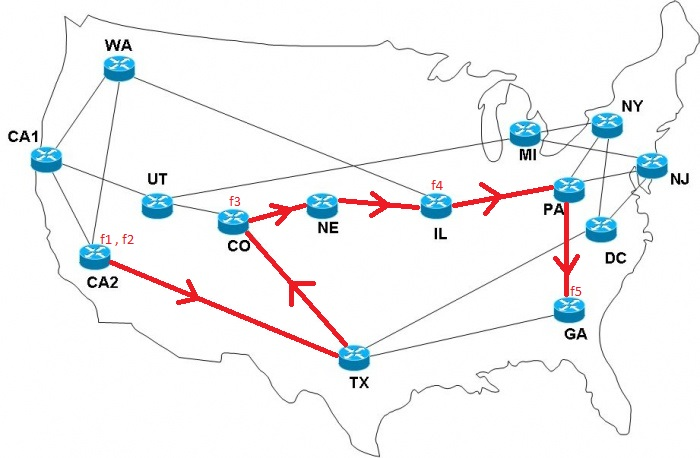
\includegraphics[scale=0.7]{nsfnet1.jpg}
\caption{One of the route and placement.}
\end{figure} 
\section{Conclusion}
We have solved the ILP problem with help of Matlab.We choose ten topologies and found optimal route and placement among of them by means of ILP solver in MATLAB. The MATLAB code is available in \emph{MATLAB} folder.
\clearpage

\addcontentsline{toc}{section}{References}
\bibliographystyle{IEEEtran}
\bibliography{IEEEabrv,ref}
\end{document}


